\section{Data Collection and Basic Analysis}
\label{sec:data}


\begin{table}[h!]
\centering
\footnotesize
{
\begin{tabular}{l|l}
\hline
Metadata Field & Explanation \\
\hline                            

{\bf size} & file size \\
{\bf type} & file type \\
{\bf tags} & labels with more specific information for each {\bf type}\\
{\bf first\_seen} & when the file was first submitted \\
{\bf last\_seen} & when the file was last submitted \\
{\bf hashes or digests} & sha1, sha256, md5, vhash, and ssdeep\\ \hline

{\bf scan\_date} & the latest scanning date for the file  \\
{\bf scan\_id} & ID of the scanning record \\
{\bf verbose\_msg} & a string for detailed scanning status \\
{\bf total} & \# of engines analyzing the file \\
{\bf positives} & \# of engines that flagged the file as malicious \\
{\bf scans} & a map containig engines' detailed analysis results \\
	\qquad {{\bf detected}} & true if the engine's label is malicious \\
	\qquad {{\bf version}}  & the version of the engine \\
	\qquad {{\bf result}}   & malware label \\
	\qquad {{\bf update}}   & the update date of the engine \\
\hline
\end{tabular}
\vspace{0.1in}
}
\mycaption{tab:fields}{VirusTotal Metadata.} 
{Fields retrieved from VirusTotal \texttt{report} and their explanation.
Some fields unrelated to this paper are not included.}
%\label{tab:fields}
\end{table}








This section introduces \vt{} and how we collect data from \vt{}. 
We also conduct simple analysis to understand 
the basic properties of our collected data. 

\subsection{\vt{}}
\vt{} is a free online malware scanning service. 
It was founded in 2004 and was acquired by google in 2012. 
\vt{} is widely used by anti-virus vendors to identify false positives and false negatives 
in their products~\cite{huangvt2016bigdata, neeles}, 
and individual users, including many academic people, 
as we discussed in Section~\ref{sec:label}.

For each submitted sample, \vt{} applies a set of anti-virus engines to analyze it. 
\vt{} keeps information about whether the submission is labeled as malware by each engine, 
and detailed tags for identified malware from each engine. 
\vt{} provides open APIs for users to interact with \vt{} 
and access the metadata of all submissions and latest detection results.
For example, \texttt{rescan} api asks \vt{} to analyze a previously submitted file again. 
\texttt{report} api returns detailed metadata and latest detection results 
for a file as shown in Table~\ref{tab:fields}. 
\texttt{distribution} api works like a pipe and keeps 
downloading information for latest submitted data from \vt{}. 



\subsection{Data Collection}

We started our data collection on August 31th, 2018. 
We randomly sampled 14423 PE files that was firstly submitted to \vt{} 
on that day using \texttt{distribution} api.
The reason we focus on PE files is that there are more 
than half of \vt{} submissions are PE files~\cite{SongAPsys2016}. 
We control our sample to have roughly 
half files labeled as benign by all vendors 
and the left half labeled as malicious by at least one vendor.
We schedule a \texttt{rescan}, and then we use \texttt{report} API to acquire
the latest detection results every day after August 31th. 
We query \texttt{report} api two hours after the scheduled \texttt{rescan} to give 
\vt{} enough time to finish the rescanning analysis. 

Our data collection still continues. 
To write this paper, we use data from August 31th, 2018 to 
November 13th, 2018 to conduct experiments in future sections. 
In total, we use data collected in consecutive 75 days. 

Due to some network issues and bugs in our code, 
we fail to get some scanning reports. 
In total, the missed reports account for less than 3\% 
of scanning reports\footnote{We should have 14432 * 75 = 1082400 scanning reports, but there are only 1050172 in our data set.}
we should get. 
Since the percentage of missed reports is low, 
we think they will not have large impact on any 
conclusion we get in future sections. 


\subsection{Basic Properties}

We conduct a set of analysis 
to learn various basic properties of our collected data.
These properties give an overview of how data set looks like
and serve as the foundation for our more 
advanced analysis in the next three sections. 

\noindent{\underline{File Properties.}}
All our sampled PE files are in 32 bit. 
Among them, 5798 are Win32 DLL files, 
and 8625 are Win32 EXE files.
For file size, more than 95\% of sampled files are 
in the range from 4KB to 4MB. 
The smallest sampled file is only 800B, 
and the largest one is larger than 389MB.

\noindent{\underline{Engine Usage Properties.}}
\vt{} applies a suite of anti-virus engines to scan submitted files.
In different scannings, used anti-virus engines may be different 
from each others. 
In total, there are 72 different engines scanning 
at least one file once in our data set. 
We conduct analysis from two aspects to 
understand how engines are used by \vt{}.

\begin{figure}[!htb]
\minipage{0.21\textwidth}
  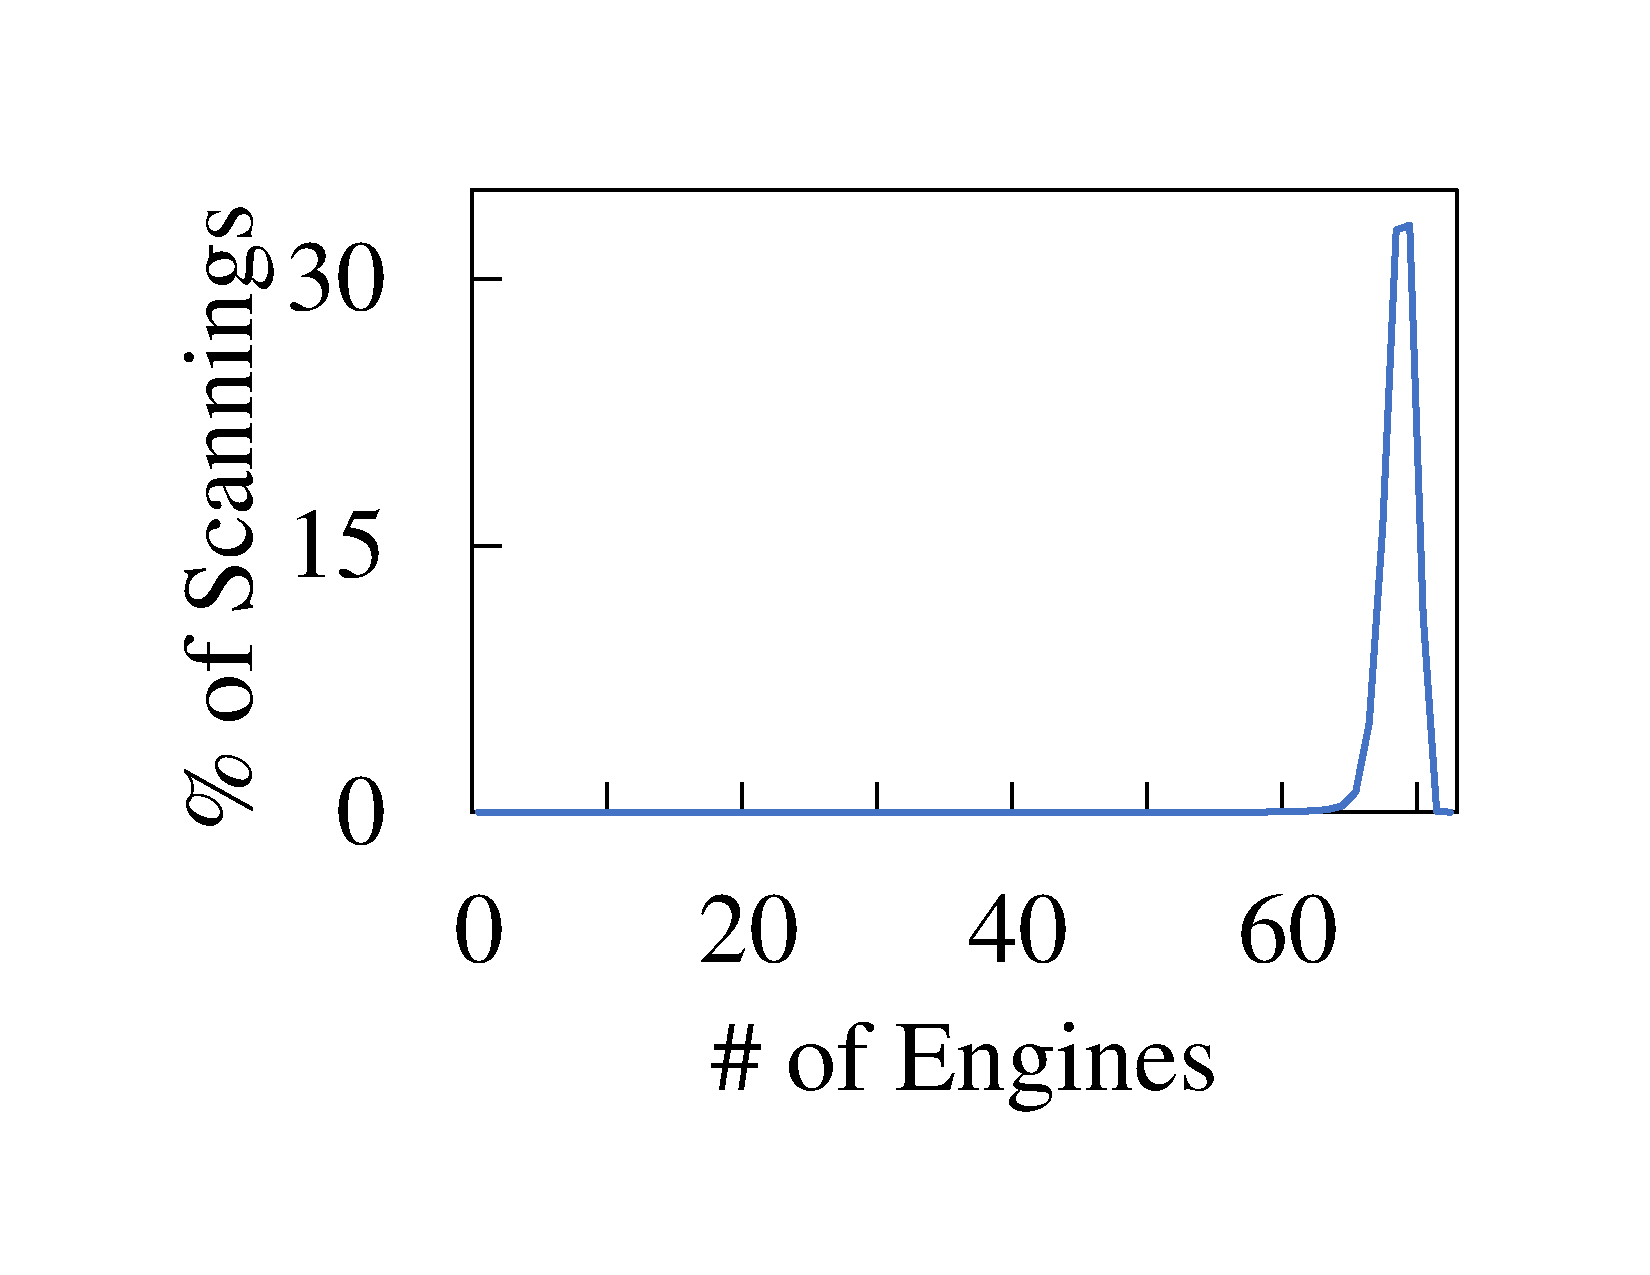
\includegraphics[width=\linewidth]{figure/vendor-scanning}
  \mycaption{fig:vendor_scanning}{How the number of engines used in one scanning distribute across all scannings.}
  {}
\endminipage\hfill
\minipage{0.21\textwidth}
  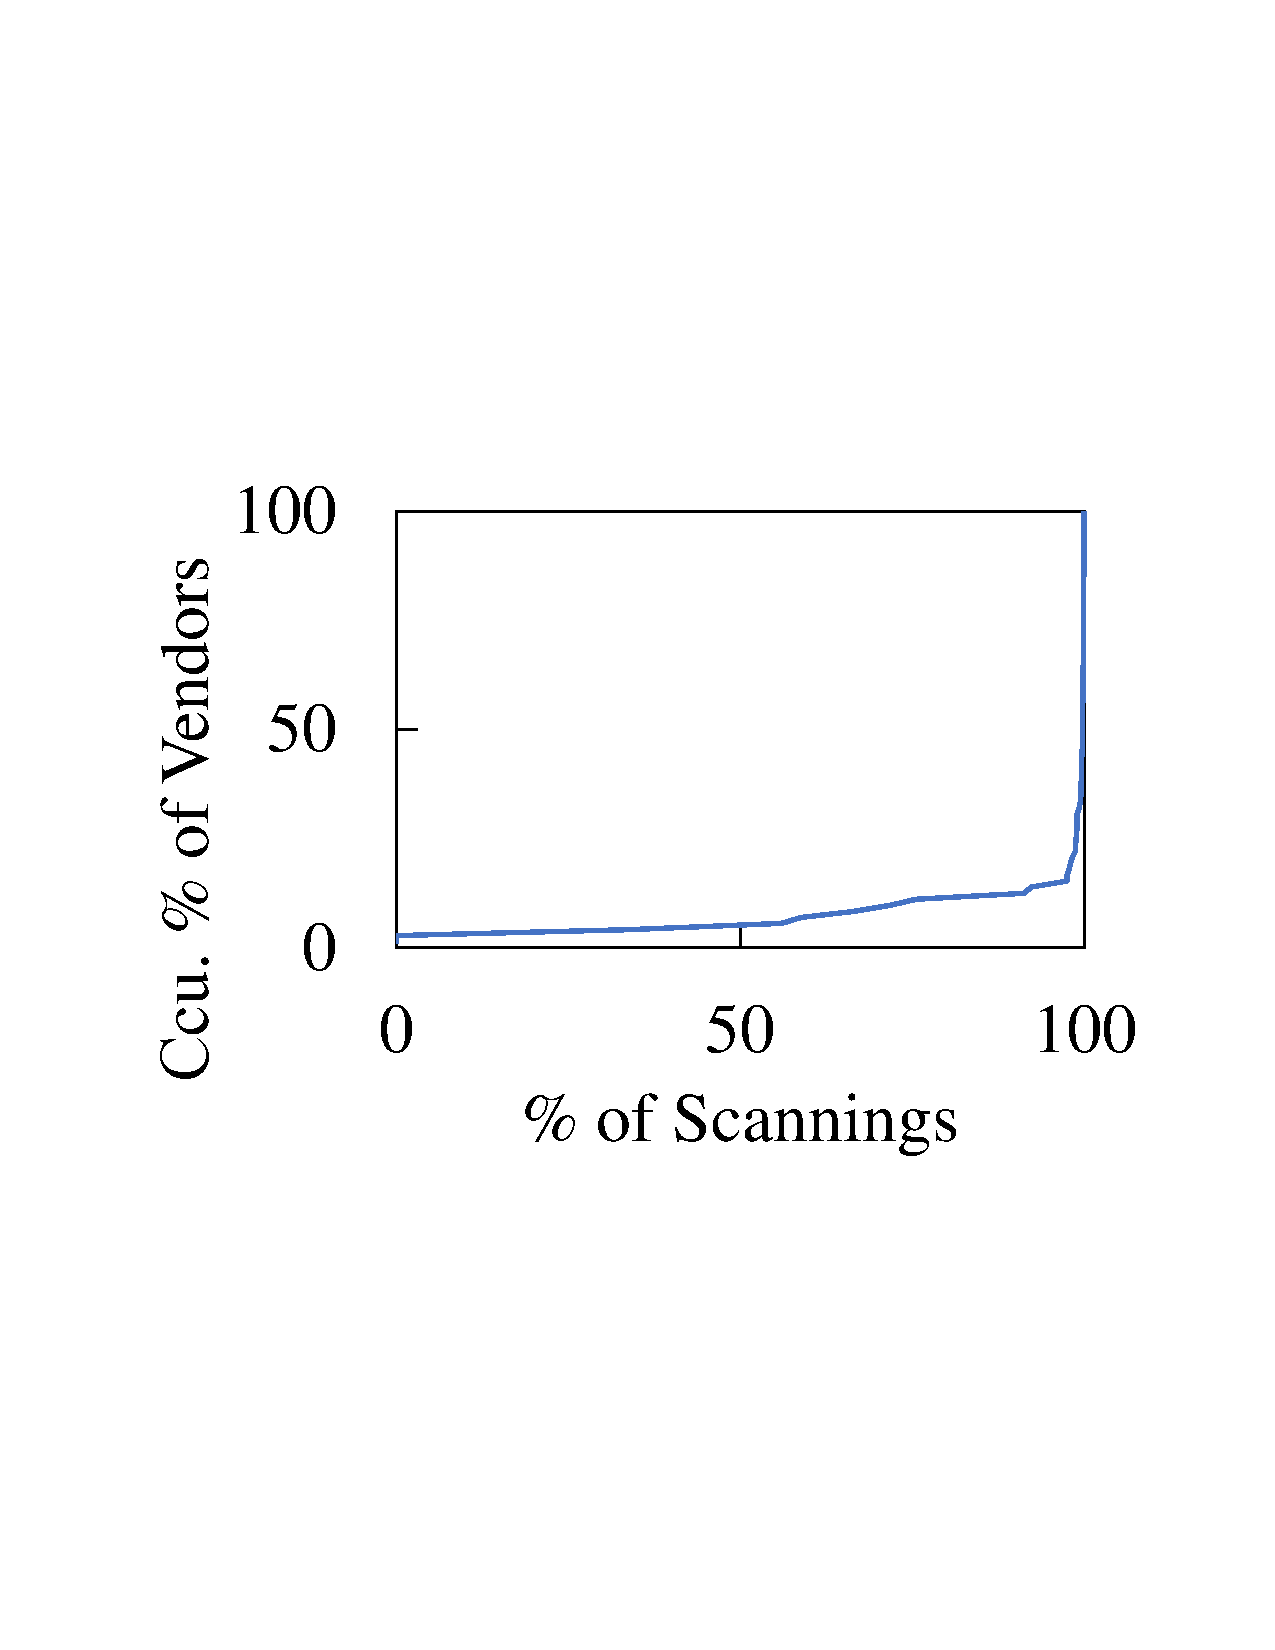
\includegraphics[width=\linewidth]{figure/scanning-vendor}
  \mycaption{fig:scanning_dis}{Cumulative \% of vendors 
over \% of scannings.}
  {Point (x, y) means y\% of vendors are used in less than x\% of scanning.}
\endminipage\hfill
\end{figure}

First, we study how many engines are used in each scanning. 
As shown in Figure~\ref{fig:vendor_scanning}, 
at least 65 engines are used in more 
than 99.11\% of scannings. 
The scannings, where less than 20 engines are used, 
are less than 0.01\%.
On average, 68.19 engines are used in one scanning. 

Second, we study how many scannings are conducted by each engine. 
Figure~\ref{fig:scanning_dis} shows how the cumulative percentage of engines changes 
over the percentage of scannings. 
64 engines are used in more than 90\% of 
the scannings in our data set. 
{\color{red} Todo: If an engine is not used frequently enough, 
we may not get meaningful conclusions for the engine. 
Therefore, in the following sections, 
we only consider the 64 engines that are used in more than 90\% of the scannings.}

\noindent{\underline{Engine Update Properties.}}
When building our data set, 
we query \vt{} every day with the 
hope to get the latest detection results from different vendors. 
One question we want to ask here is whether a more recent scanning 
is really conducted by more recent versions of engines. 
As shown in Table~\ref{tab:fields},
\vt{} provide the information about when 
an engine is updated for each scanning.  
To answer the question, we sort scannings conducted by the same engine 
on the same file chronologically.
For every pair of consecutive scannings, we compare their update information. 
More than 78\% of consecutive pairs, the update date for the later scanning is more recent.
More than {\color{red} xx\%} of consecutive pairs, the update date of the later 
scanning is not earlier than the previous scanning. 
Overall, more recent scannings are largely conducted
by more recent versions of engines. 

We also study the update frequency for different engines. 
Different engines have different update frequency. 
{\color{red} TODO}. 

\subsection{Discussion}

{\color{red} TODO}